\subsubsection{Peak Features}
The \textit{Peak Features}-tool calculates the expected position of gamma spectrum features from a known photopeak energy. The features can then be marked with lines in the \textit{Spectrum}-tab.

\begin{figure}[H]
    \centering
    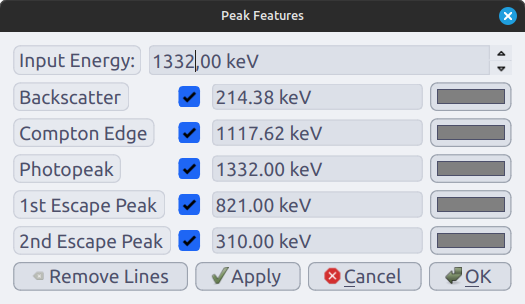
\includegraphics[width = .4\linewidth]{images/interface/peak_features.png}
    \caption{Peak Features tool with the \qty{1332}{\kilo\electronvolt} energy of Co-60 set.}
    \label{fig:peak_features}
    \begin{flushleft}
        \begin{itemize}
            \item \texttt{Remove Lines}: Removed and lines placed in the \textit{Spectrum}-tab.
            \item \texttt{Apply}: Adds lines to the \textit{Spectrum}-tab.
            \item \texttt{Cancel}: Closes the dialog with no other action taken.
            \item \texttt{Ok}: Applies the lines and closes the dialog.
        \end{itemize}
    \end{flushleft}
\end{figure}